\documentclass[12pt]{article}
\usepackage[utf8]{inputenc}
\usepackage{graphicx}
\graphicspath{{images/}}
\begin{document}
\begin{center}
\huge\underline{`Solutions to Covid-19 Provided by}
\huge\underline{ Biomedical Engineers''}
\end{center}
\begin{center}
 
\includegraphics[scale=0.8]{nitlogo.png }
\end{center}
\vspace{1cm}
\begin{center}
   \emph{\large By}\\
\Large{Raj Motwani }\\
\large{Roll No- 21111042}\\
\large{Biomedical 1st Sem}\\
\end{center}
\clearpage
\section{Adapting to help the NHS}

\includegraphics[scale=0.4]{nhs.png}\\
Biomedical Engineers from a range of industry backgrounds have been putting their normal tasks to one side to build ventilators and PPE (personal protection equipment) to help the NHS care for the increasing numbers of patients in Intensive Care Units with COVID-19. 
\\

They are using their ingenuity to make the items that are so desperately needed. Many are using reverse engineering techniques to help them to deconstruct items and their parts to help them better understand the make-up of the equipment and the optimum methods needed to recreate them. This process would normally take many months, but the challenge now is to shorten this time frame as much as possible. Items are needed within days or weeks, so they are working to safely speed up the production and testing process, to ensure that equipment is distributed quickly, while still meeting high health and safety requirements such as sterilisation measures set out by the Medicines and Healthcare Products Regulatory Agency (MHRA).
\\

One of the many processes used in manufacturing is 3D printing. This is a useful tool for engineers, as it allows them to make copies of precise items several times over. In response to the COVID-19 outbreak, many small companies or individuals with access to 3D printers are doing their part to produce additional face masks and visors for healthcare workers, and those working in close proximity to other people.


Airbus, Apple, Babcock, Dyson, Mercedes Formula 1, Tesla and Vauxhall are just some of the big name companies that are currently helping bridge the gap in supply, and some are following specifications provided by the Government to make the process as efficient as possible.

\section{Ventilators}
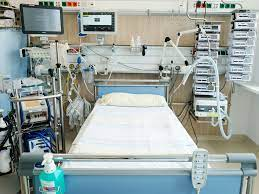
\includegraphics[scale=0.7]{ven.jpeg}\\
Patients who cannot breathe spontaneously need to be put on a ventilator. Ventilators are capable of replacing the breath function and patients in an advanced state of respiratory distress are usually intubated and sedated at the beginning of the treatment.


Ventilators are capable of replacing the breath function and patients in an advanced state of respiratory distress are usually intubated and sedated at the beginning of the treatment. They are complex systems providing the healthcare professionals with a lot of flexibility to adapt the assisted breathing settings and to be able to wean recovering patients off the ventilator gradually.

Modern ventilators are typically closed loop pressure controlled and capable of detecting spontaneous breathing to synchronise assistance for recovering patients. They also enable the control of the composition of the gas the patient breathes from normal air to 100 percent oxygen, usually taking their supply from the hospital’s gas supply network but can also be coupled to oxygen tanks or oxygen concentrators if used in a setting where there is no gas network.

\section{Biomedical Engineers’ rapid response to PPE needs}
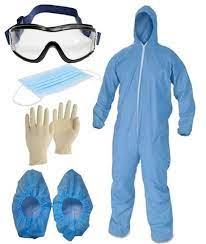
\includegraphics[scale=0.7]{ppe.jpeg}\\
According to infectious disease experts, face shields protect the face from fluids, spray, and droplets, while extending the life of N95 face masks.
\\
The COVID-19 pandemic has depleted supplies of personal protective equipment (PPE) for healthcare professionals nationwide. Dr. Karilyn Larkin is a hematologist at The Ohio State University Comprehensive Cancer Center – Arthur G. James Cancer Hospital and Richard J. Solove Research Institute. When she and her colleagues experienced shortages of face shields, she turned to Ohio State engineers—specifically Mechanical and Aerospace Engineering Professor Carlos Castro—for help 3D printing face shields.

\section{Pivoting to vaccines}
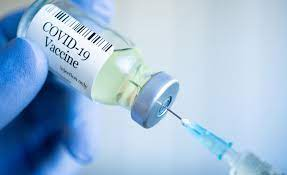
\includegraphics[scale=0.6]{vac.jpeg}\\
The labs of Biomedical Engineering Professors Daniel Gallego-Perez and Natalia Higuita-Castro are developing novel, highly benign and targeted methods for the delivery of mRNA vaccines. While the researchers normally focus on cancer and regenerative medicine, their methods may be applicable to vaccine development and deployment.
\section{Solution to Health Disparities}
A systems approach to health disparities by engineers affords a special opportunity to merge the development of innovative technologies with unmet health needs fueled by structural racism and social determinants of health. Without a lens through which inequities that shape disease processes and access to care, designs that are accessible and fully effective for all populations will be lacking. Collaborations between engineers and clinicians through clinically centered experiences—also known as clinical immersion and biodesign—allows for the collaborative identification of unmet needs and pursuit of technical solutions to meet those needs. This can be done in a number of training settings ranging from courses co-led by engineering and medical schools to intensive short-term programs. The author has led a program called Coulter College funded by the Wallace H. Coulter Foundation and recently hosted by Medtronic. During an intensive 3-day program focused on the translation of biomedical innovations, student teams are guided through a dynamic process to develop solutions to clinical needs while gaining a better understanding of resource constraints and disparities that must be considered during the design process. Students learn how to evaluate the best point of leverage within a given clinical need, how to evaluate solutions, and how to balance clinical benefits alongside a viable commercial model. Efforts like Coulter College and training that combines clinical immersion and biodesign will benefit from expansion and a constant focus on underserved disparity populations.



\enddocument